\documentclass[12pt,preprint]{elsarticle}

\usepackage{lmodern}
%%%% My spacing
\usepackage{setspace}
\setstretch{1.2}
\DeclareMathSizes{12}{14}{10}{10}

% Wrap around which gives all figures included the [H] command, or places it "here". This can be tedious to code in Rmarkdown.
\usepackage{float}
\let\origfigure\figure
\let\endorigfigure\endfigure
\renewenvironment{figure}[1][2] {
    \expandafter\origfigure\expandafter[H]
} {
    \endorigfigure
}

\let\origtable\table
\let\endorigtable\endtable
\renewenvironment{table}[1][2] {
    \expandafter\origtable\expandafter[H]
} {
    \endorigtable
}


\usepackage{ifxetex,ifluatex}
\usepackage{fixltx2e} % provides \textsubscript
\ifnum 0\ifxetex 1\fi\ifluatex 1\fi=0 % if pdftex
  \usepackage[T1]{fontenc}
  \usepackage[utf8]{inputenc}
\else % if luatex or xelatex
  \ifxetex
    \usepackage{mathspec}
    \usepackage{xltxtra,xunicode}
  \else
    \usepackage{fontspec}
  \fi
  \defaultfontfeatures{Mapping=tex-text,Scale=MatchLowercase}
  \newcommand{\euro}{€}
\fi

\usepackage{amssymb, amsmath, amsthm, amsfonts}

\def\bibsection{\section*{References}} %%% Make "References" appear before bibliography


\usepackage[numbers]{natbib}

\usepackage{longtable}
\usepackage[margin=2.3cm,bottom=2cm,top=2.5cm, includefoot]{geometry}
\usepackage{fancyhdr}
\usepackage[bottom, hang, flushmargin]{footmisc}
\usepackage{graphicx}
\numberwithin{equation}{section}
\numberwithin{figure}{section}
\numberwithin{table}{section}
\setlength{\parindent}{0cm}
\setlength{\parskip}{1.3ex plus 0.5ex minus 0.3ex}
\usepackage{textcomp}
\renewcommand{\headrulewidth}{0.2pt}
\renewcommand{\footrulewidth}{0.3pt}

\usepackage{array}
\newcolumntype{x}[1]{>{\centering\arraybackslash\hspace{0pt}}p{#1}}

%%%%  Remove the "preprint submitted to" part. Don't worry about this either, it just looks better without it:
\makeatletter
\def\ps@pprintTitle{%
  \let\@oddhead\@empty
  \let\@evenhead\@empty
  \let\@oddfoot\@empty
  \let\@evenfoot\@oddfoot
}
\makeatother

 \def\tightlist{} % This allows for subbullets!

\usepackage{hyperref}
\hypersetup{breaklinks=true,
            bookmarks=true,
            colorlinks=true,
            citecolor=blue,
            urlcolor=blue,
            linkcolor=blue,
            pdfborder={0 0 0}}


% The following packages allow huxtable to work:
\usepackage{siunitx}
\usepackage{multirow}
\usepackage{hhline}
\usepackage{calc}
\usepackage{tabularx}
\usepackage{booktabs}
\usepackage{caption}


\newenvironment{columns}[1][]{}{}

\newenvironment{column}[1]{\begin{minipage}{#1}\ignorespaces}{%
\end{minipage}
\ifhmode\unskip\fi
\aftergroup\useignorespacesandallpars}

\def\useignorespacesandallpars#1\ignorespaces\fi{%
#1\fi\ignorespacesandallpars}

\makeatletter
\def\ignorespacesandallpars{%
  \@ifnextchar\par
    {\expandafter\ignorespacesandallpars\@gobble}%
    {}%
}
\makeatother


% definitions for citeproc citations
\NewDocumentCommand\citeproctext{}{}
\NewDocumentCommand\citeproc{mm}{%
\href{\#cite.\detokenize{#1}}{#2}\nocite{#1}}

\makeatletter
% allow citations to break across lines
\let\@cite@ofmt\@firstofone
% avoid brackets around text for \cite:
\def\@biblabel#1{}
\def\@cite#1#2{{#1\if@tempswa , #2\fi}}
\makeatother
\newlength{\cslhangindent}
\setlength{\cslhangindent}{1.5em}
\newlength{\csllabelwidth}
\setlength{\csllabelwidth}{3em}
\newenvironment{CSLReferences}[2] % #1 hanging-indent, #2 entry-spacing
{\begin{list}{}{%
	\setlength{\itemindent}{0pt}
	\setlength{\leftmargin}{0pt}
	\setlength{\parsep}{0pt}
	% turn on hanging indent if param 1 is 1
	\ifodd #1
	\setlength{\leftmargin}{\cslhangindent}
	\setlength{\itemindent}{-1\cslhangindent}
	\fi
	% set entry spacing
	\setlength{\itemsep}{#2\baselineskip}}}
{\end{list}}

\usepackage{calc}
\newcommand{\CSLBlock}[1]{\hfill\break\parbox[t]{\linewidth}{\strut\ignorespaces#1\strut}}
\newcommand{\CSLLeftMargin}[1]{\parbox[t]{\csllabelwidth}{\strut#1\strut}}
\newcommand{\CSLRightInline}[1]{\parbox[t]{\linewidth - \csllabelwidth}{\strut#1\strut}}
\newcommand{\CSLIndent}[1]{\hspace{\cslhangindent}#1}


\urlstyle{same}  % don't use monospace font for urls
\setlength{\parindent}{0pt}
\setlength{\parskip}{6pt plus 2pt minus 1pt}
\setlength{\emergencystretch}{3em}  % prevent overfull lines
\setcounter{secnumdepth}{5}

%%% Use protect on footnotes to avoid problems with footnotes in titles
\let\rmarkdownfootnote\footnote%
\def\footnote{\protect\rmarkdownfootnote}
\IfFileExists{upquote.sty}{\usepackage{upquote}}{}

%%% Include extra packages specified by user

%%% Hard setting column skips for reports - this ensures greater consistency and control over the length settings in the document.
%% page layout
%% paragraphs
\setlength{\baselineskip}{12pt plus 0pt minus 0pt}
\setlength{\parskip}{12pt plus 0pt minus 0pt}
\setlength{\parindent}{0pt plus 0pt minus 0pt}
%% floats
\setlength{\floatsep}{12pt plus 0 pt minus 0pt}
\setlength{\textfloatsep}{20pt plus 0pt minus 0pt}
\setlength{\intextsep}{14pt plus 0pt minus 0pt}
\setlength{\dbltextfloatsep}{20pt plus 0pt minus 0pt}
\setlength{\dblfloatsep}{14pt plus 0pt minus 0pt}
%% maths
\setlength{\abovedisplayskip}{12pt plus 0pt minus 0pt}
\setlength{\belowdisplayskip}{12pt plus 0pt minus 0pt}
%% lists
\setlength{\topsep}{10pt plus 0pt minus 0pt}
\setlength{\partopsep}{3pt plus 0pt minus 0pt}
\setlength{\itemsep}{5pt plus 0pt minus 0pt}
\setlength{\labelsep}{8mm plus 0mm minus 0mm}
\setlength{\parsep}{\the\parskip}
\setlength{\listparindent}{\the\parindent}
%% verbatim
\setlength{\fboxsep}{5pt plus 0pt minus 0pt}



\begin{document}



\begin{frontmatter}  %

\title{Rethinking Market Cap Dynamics: A South African Perspective on
Risk and Return}

% Set to FALSE if wanting to remove title (for submission)




\author[Add1]{Hendri van Zyl}
\ead{17640296@sun.ac.za}

\author[Add2]{Nico Katzke}
\ead{nfkatzke.class@gmail.com}




\address[Add1]{Stellenosch University, South Africa}
\address[Add2]{Satrix, Cape Town, South Africa}



\vspace{1cm}





\vspace{0.5cm}

\end{frontmatter}

\setcounter{footnote}{0}



%________________________
% Header and Footers
%%%%%%%%%%%%%%%%%%%%%%%%%%%%%%%%%
\pagestyle{fancy}
\chead{}
\rhead{}
\lfoot{}
\rfoot{\footnotesize Page \thepage}
\lhead{}
%\rfoot{\footnotesize Page \thepage } % "e.g. Page 2"
\cfoot{}

%\setlength\headheight{30pt}
%%%%%%%%%%%%%%%%%%%%%%%%%%%%%%%%%
%________________________

\headsep 35pt % So that header does not go over title




\section{\texorpdfstring{Introduction
\label{Introduction}}{Introduction }}\label{introduction}

This study examines whether smaller stocks exhibit greater stability
than larger ones by analysing volatility differences across small, mid,
and large-cap stocks listed on the Johannesburg Stock Exchange (JSE).
Financial theory suggests that small-cap stocks are typically more
volatile due to higher risk exposure, lower liquidity, and greater
sensitivity to economic conditions. Jena, Tiwari, Dash \& Aikins Abakah
(\citeproc{ref-jena2021volatility}{2021}) point out that despite the
unconditional correlation between these indices, they exhibit very
different risk, return and liquidity profiles. Moreover, their findings
indicate that in India, large cap stocks offer investors an opportunity
for diversification and hedging in the short and long run, respectively.
By splitting the JSE All Share Index (J203) into three market cap
segments and weighting them by market capitalization, this analysis
provides a clearer understanding of how volatility varies across stock
sizes.

To measure stability and risk, the study examines rolling 3-year
standard deviations, Sharpe ratios, maximum drawdowns, and correlations
with the J203 index to assess systematic risk exposure. These metrics
provide insight into the risk-return trade-off for each segment and
allow for a simple comparison of volatility dynamics. Though limited in
scope this research can illuminate the differences in stability across
market capitalisation and whether this dimension presents an opportunity
for portfolio diversification.

\section{\texorpdfstring{Data \label{Data}}{Data }}\label{data}

This analysis utilizes data from the JSE All Share Index (J203),
covering daily returns and proportional weights of 99\% of JSE-listed
stocks from January 1, 2014, to November 29, 2024. Instead of analysing
individual stocks, the dataset was aggregated and reweighted based on
market capitalization classifications at each point in time. This means
that stocks were dynamically grouped into small, mid, and large-cap
categories as their market cap evolved over the period. Consequently,
the units of observation in this study are the market cap-weighted
indices for small, mid, and large-cap stocks, allowing for a structured
comparison of their volatility, performance, and risk dynamics over
time. Additionally, for comparative purposes, the 2-year South African
bond yield is included as a benchmark. However, it is important to note
that the last available bond yield data is from March 2022, meaning that
all direct comparisons are limited to this period. A summary of the
returns data is provided in Table 2.1 below. Notably, small caps exhibit
the lowest standard deviation, suggesting relatively lower volatility
compared to mid and large caps. Interestingly, the bond yield displays
extreme kurtosis and negative skewness, indicating the presence of rare
but severe fluctuations, which contrast with the more moderate
distribution of equity returns. The results of the comparisons are
provided in the next section.

\begin{table}[H]
    \centering
    \caption{Descriptive Statistics for Market Cap Indices and Bond Yields}
    \label{tab:tablestats}
    \begin{tabular}{lcccc}
        \hline
        Statistic & Small Caps & Mid Caps & Large Caps & Bond 2Y \\
        \hline
        Observations & 2061.000 & 2061.000 & 2061.000 & 2061.000 \\
        NAs & 0.000 & 0.000 & 0.000 & 0.000 \\
        Minimum & -0.092 & -0.087 & -0.100 & -0.261 \\
        Quartile 1 & -0.004 & -0.005 & -0.006 & -0.003 \\
        Median & 0.001 & 0.001 & 0.001 & 0.000 \\
        Arithmetic Mean & 0.000 & 0.000 & 0.000 & 0.000 \\
        Geometric Mean & 0.000 & 0.000 & 0.000 & 0.000 \\
        Quartile 3 & 0.005 & 0.006 & 0.007 & 0.003 \\
        Maximum & 0.075 & 0.062 & 0.086 & 0.157 \\
        SE Mean & 0.000 & 0.000 & 0.000 & 0.000 \\
        LCL Mean (0.95) & 0.000 & 0.000 & 0.000 & 0.000 \\
        UCL Mean (0.95) & 0.001 & 0.001 & 0.001 & 0.000 \\
        Variance & 0.000 & 0.000 & 0.000 & 0.000 \\
        Stdev & 0.009 & 0.011 & 0.012 & 0.011 \\
        Skewness & -0.967 & -0.814 & -0.409 & -3.885 \\
        Kurtosis & 19.821 & 9.526 & 7.042 & 207.480 \\
        \hline
    \end{tabular}
\end{table}

\section{Results}\label{results}

Figure 3.1 presents the cumulative returns of the market cap-weighted
indices over the sample period. From 2014 to 2020, the performance of
small, mid, and large-cap indices remained relatively similar, with no
significant divergence among them. However, following the COVID-19
pandemic and the subsequent market recovery, small-cap stocks
demonstrated a clear outperformance compared to mid and large caps. This
suggests that, while all segments were impacted by the initial market
shock, small caps experienced a stronger post-pandemic rebound,
potentially driven by sector-specific recoveries. This divergence
highlights the differing market dynamics across capitalization sizes in
response to economic shocks and recoveries.

\begin{figure}[H]

{\centering 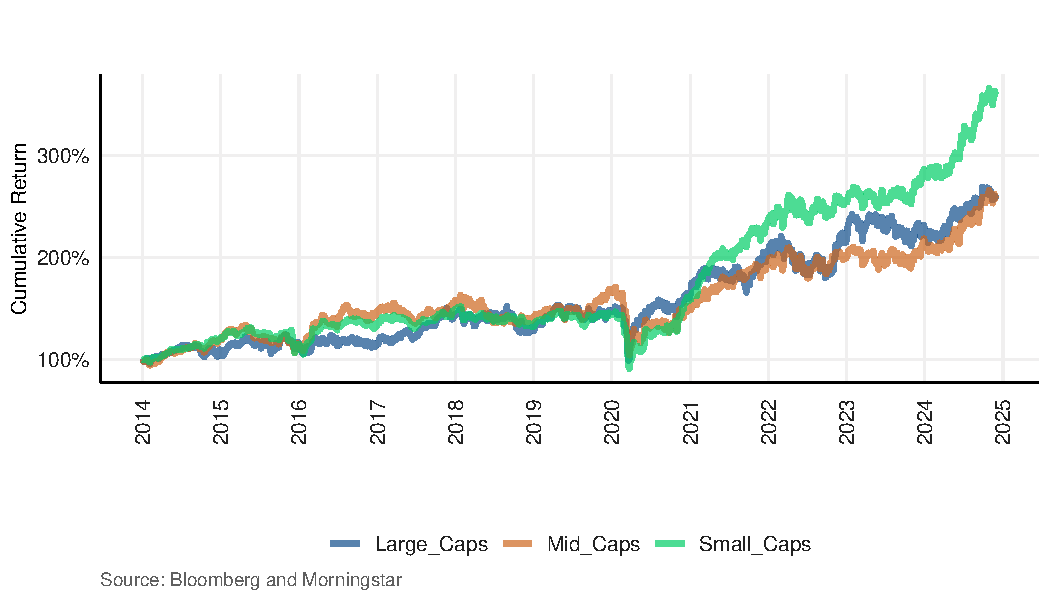
\includegraphics{plots/cum_plot} 

}

\caption{Cumulative Returns by Market Cap Size \label{Figure1}}\label{fig:Figure1}
\end{figure}

Figure 3.2 illustrates the annualized 3-year rolling returns for the
market cap indices. The results reinforce the earlier observation that
small-cap stocks often delivered superior returns throughout the
majority of the sample period. Unlike cumulative returns, where small
caps only began to notably outperform after the COVID-19 recovery, the
rolling return data suggests that small caps maintained a persistent
performance advantage over mid and large caps for nearly the entire
sample range.

This trend highlights the long-term return premium potentially
associated with smaller stocks, this could reflect higher growth
potential, greater market inefficiencies, or increased risk-taking by
investors in certain periods. By the final years of the sample, however,
the rolling returns of large caps began to converge with those of small
caps, suggesting a possible stabilization in market dynamics or a shift
in investor preference towards larger, more established companies.

\begin{figure}[H]

{\centering 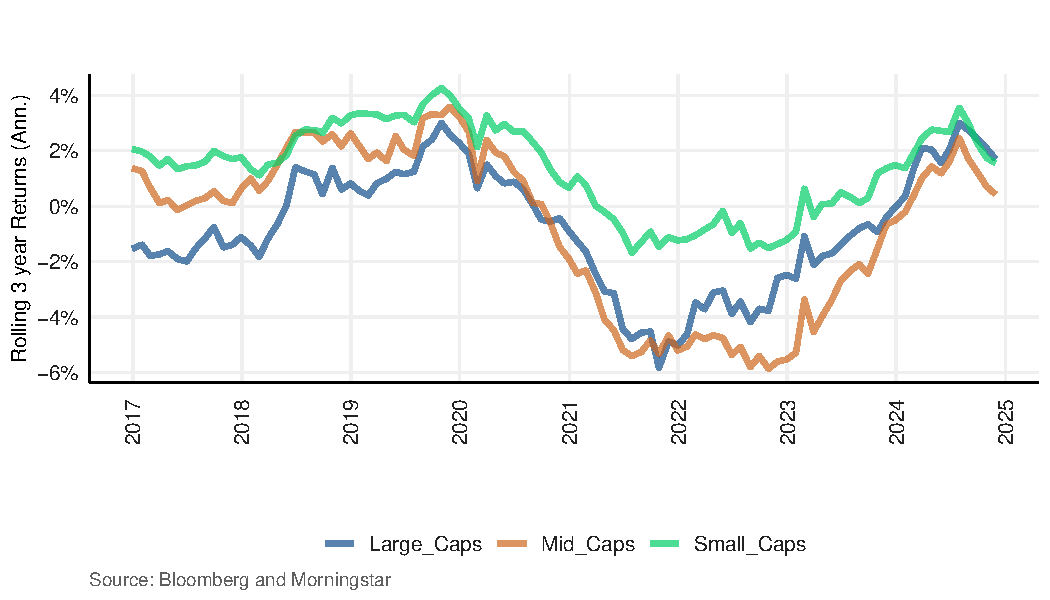
\includegraphics{plots/ret_plot} 

}

\caption{Annualized 3-year Rolling Returns By Market Cap Size \label{Figure2}}\label{fig:Figure2}
\end{figure}

Figure 3.3 presents the annualized 3-year rolling standard deviation for
the market cap indices, highlighting a counterintuitive finding: small
caps exhibit a consistently lower standard deviation compared to both
mid and large caps throughout the sample period. This result challenges
conventional financial theory, which typically associates small caps
with higher volatility due to their lower liquidity, greater sensitivity
to market shocks, and heightened exposure to idiosyncratic risks.

Interestingly, mid and large caps display relatively similar volatility
levels for much of the sample, with only small deviations until 2023.
After this point, mid caps experience a noticeable decline in standard
deviation, bringing their volatility closer to that of small caps, while
large caps maintain relatively stable volatility. The relative stability
of small caps raises questions about the underlying drivers of their
performance and volatility. This finding emphasizes the need for further
investigation into the volatility drivers and risk-return tradeoffs
within small-cap stocks, as they appear to defy traditional expectations
over this sample period.

\begin{figure}[H]

{\centering 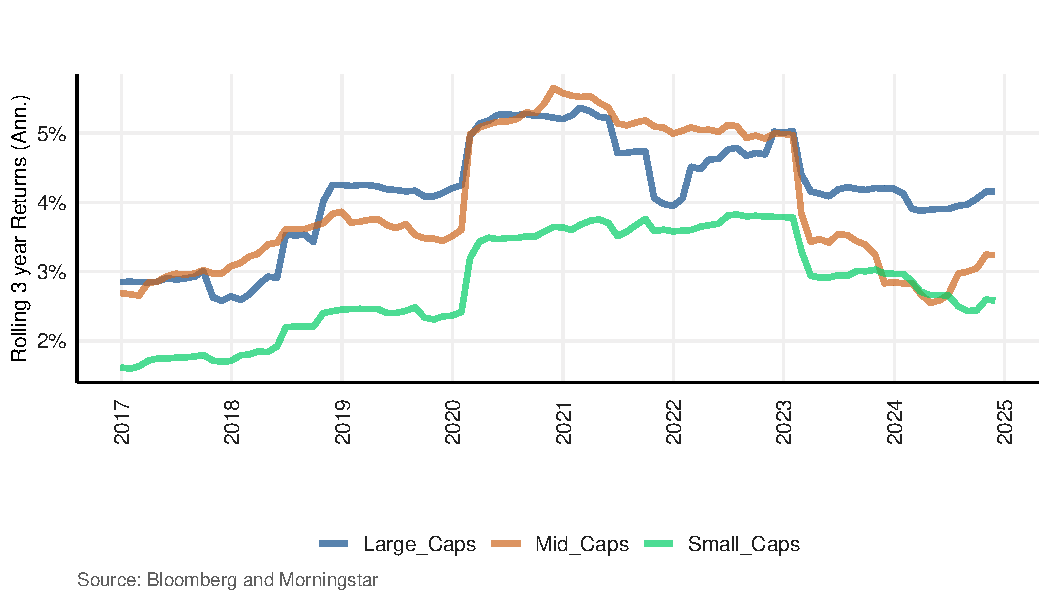
\includegraphics{plots/sd_plot} 

}

\caption{Annualized 3-year Rolling SD By Market Cap Size \label{Figure3}}\label{fig:Figure3}
\end{figure}

The table summarises downside risk estimates for small and mid-cap
stocks, focusing on metrics that quantify potential losses and tail
risks. While results for large caps appear to be incorrect here, the
comparison between small and mid caps can still provide meaningful
insights. Mid caps consistently exhibit higher risk than small caps,
with higher semi-deviation (0.76\% vs.~0.65\%) and downside deviation
(0.74\% vs.~0.63\%), indicating greater variability and downside
exposure during periods of negative returns. Furthermore, mid caps show
only a slightly smaller maximum drawdown (39.07\%) than small caps
(40.26\%), suggesting comparable responses during extreme market
downturns.

When assessing tail risks using Value at Risk (VaR) and Expected
Shortfall (ES), mid caps exhibit the highest downside exposure, with a
Historical VaR (95\%) of -1.53\% and ES of -2.33\%, compared to small
caps (-1.21\% and -1.97\%). This pattern persists when adjusting for
non-normal return distributions: mid caps have a Modified VaR (95\%) of
-1.68\% and Modified ES (95\%) of -3.54\%, compared to -1.29\% and
-2.32\% for small caps. These results suggest that mid caps are more
vulnerable to extreme downside events, possibly reflecting a greater
sensitivity to market shocks or less consistent investor demand relative
to small caps.

Overall, small caps exhibit lower overall risk than mid caps across most
downside risk measures, with lower deviations, VaR, and ES. However,
both categories show significant exposure to extreme tail events,
underscoring the inherent risks associated with smaller-cap segments of
the market.

\begin{figure}[H]

{\centering 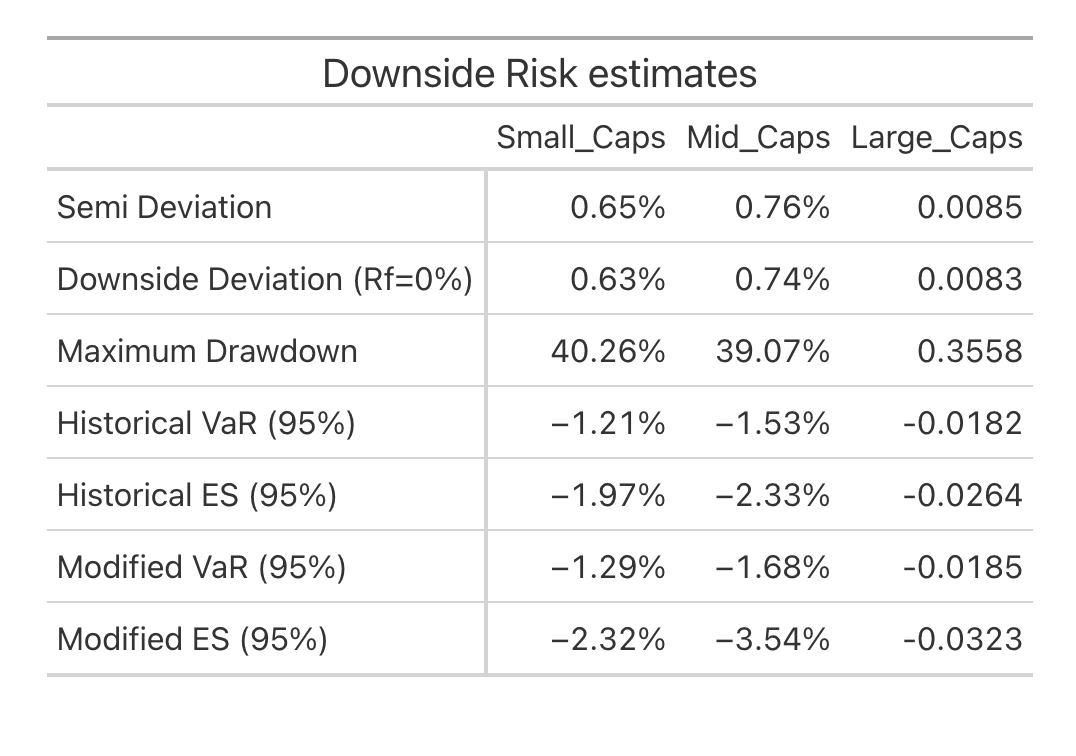
\includegraphics[width=0.8\linewidth]{tables/downside} 

}

\caption{Table 1: Risk Measures \label{tab:Table1}}\label{fig:Table1}
\end{figure}

Table 2 below provides a 5-year comparative analysis of the performance
and risk metrics for small, mid, and large-cap stocks, along with the
2-year South African bond yield (Bond\_2Y), although its results appear
to be wrong to will be ignored. Over the past five years, small caps
have delivered the highest cumulative returns (79.4\%), outperforming
both large caps (76.8\%) and mid caps (39.5\%). Small caps also
generated the highest excess returns above the benchmark (20.5\%),
slightly edging out large caps (20.2\%). Mid caps lagged significantly,
with cumulative returns of 39.5\% and excess returns of 14.5\%. These
results highlight the superior long-term performance of small caps
compared to other market segments. The statistics for the 2-year bond
yield, however, appear to be incorrect and have been excluded from the
analysis.

In terms of risk, large caps exhibited the highest annualized standard
deviation (4.4\%), followed closely by mid caps (4.1\%), while small
caps (3.6\%) were the least volatile. Despite their higher volatility,
large caps delivered the best risk-adjusted performance, as indicated by
their superior Adjusted Sharpe Ratio (0.493) compared to mid caps
(0.327) and small caps (0.302). Downside risk metrics reveal that mid
caps were the most vulnerable, with the largest average drawdown (4.2\%)
and the highest Modified CVaR (-0.047). Small caps, while maintaining
lower volatility, also showed better downside protection, with a lower
average drawdown (2.6\%) and Modified CVaR (-0.041) compared to mid
caps. Large caps demonstrated strong performance on downside metrics
also with a moderate drawdown (3.8\%) and Modified CVaR (-0.042).

Market sensitivity further distinguishes these indices. Small caps had
the highest Information Ratio (0.762), reflecting their superior
risk-adjusted excess returns relative to the benchmark, while mid caps
trailed with an Information Ratio of 0.498. In bear markets, large caps
(-0.060) exhibited greater stability, with a lower downside beta than
small caps (-0.070) and mid caps (-0.041). This highlights the ability
of large caps to better weather market downturns. Overall, this analysis
underscores the strong risk-return trade-off of small caps, the greater
vulnerability of mid caps, and the consistent risk-adjusted performance
of large caps, offering valuable insights for portfolio diversification
and risk management.

\begin{figure}[H]

{\centering 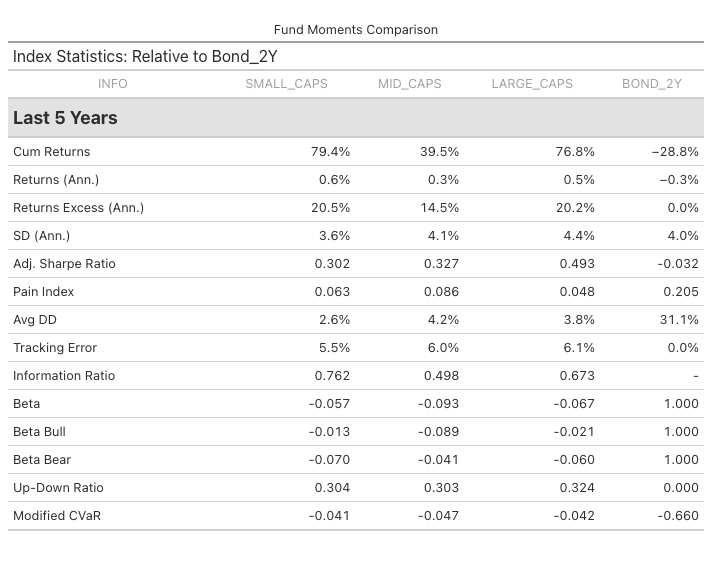
\includegraphics[width=0.8\linewidth]{tables/comp} 

}

\caption{Table 2: Descriptive Statistics \label{tab:Table2}}\label{fig:Table2}
\end{figure}

\section{Conclusion}\label{conclusion}

This analysis highlights the distinct performance and risk dynamics of
small, mid, and large-cap stocks on the Johannesburg Stock Exchange over
the past 5 years. Small caps emerged as the strongest performer,
delivering superior long-term returns and maintaining relatively
moderate volatility. Their consistent outperformance highlights their
potential for yielding higher growth, even while exhibiting less
downside risks. In contrast, mid caps proved to be the most vulnerable
segment, struggling with lower returns and higher exposure to market
shocks, as reflected in their risk metrics.

Large caps demonstrated a balance between return and risk, offering
competitive performance while maintaining greater stability during
adverse market conditions. They provided strong risk-adjusted returns,
emphasizing their appeal to more risk-averse investors. Overall, the
findings suggest that small caps are well-suited for those seeking
higher growth with manageable risk, while large caps provide a stable
and reliable option. These findings challenge the mainstream notion that
small caps are inherently more volatile and riskier than their larger
counterparts. A deeper investigation is required to better understand
the underlying factors driving this unique behaviour in the South
African market, such as structural differences, sectoral composition, or
local economic dynamics.

\newpage

\section*{References}\label{references}
\addcontentsline{toc}{section}{References}

\phantomsection\label{refs}
\begin{CSLReferences}{1}{1}
\bibitem[\citeproctext]{ref-jena2021volatility}
Jena, S.K., Tiwari, A.K., Dash, A. \& Aikins Abakah, E.J. 2021.
Volatility spillover dynamics between large-, mid-, and small-cap stocks
in the time-frequency domain: Implications for portfolio management.
\emph{Journal of Risk and Financial Management}. 14(11):531.

\end{CSLReferences}

\bibliography{Tex/ref}





\end{document}
